\begin{comment}
\documentclass[10pt]{article}
\usepackage{fullpage, graphicx, url}
\setlength{\parskip}{1ex}
\setlength{\parindent}{0ex}
\title{FLbox}
\begin{document}


\begin{tabular}{ccc}
The Alternative Csound Reference Manual & & \\
Previous & &Next

\end{tabular}

%\hline 
\end{comment}
\section{FLbox}
FLbox�--� A FLTK widget that displays text inside of a box. \subsection*{Description}


  A FLTK widget that displays text inside of a box. 
\subsection*{Syntax}


 ihandle \textbf{FLbox}
 ``label'', itype, ifont, isize, iwidth, iheight, ix, iy [, image]
\subsection*{Initialization}


 \emph{ihandle}
 -- a handle value (an integer number) that unequivocally references a corresponding widget. This is used by other opcodes that modify a widget's properties (see \emph{Modifying FLTK Widget Appearance}
). It is automatically output by \emph{FLbox}
 and must not be set by the user label. (The user label is a double-quoted string containing some user-provided text placed near the widget.) 


 \emph{``label''}
 -- a double-quoted string containing some user-provided text, placed near corresponding widget. 


  Notice that with \emph{FLbox}
, it is not necessary to call the \emph{FLsetTextType}
 opcode at all in order to use a symbol. In this case, it is sufficient to set a label starting with ``@'' followed by the proper formatting string. 


  The following symbols are supported: 


 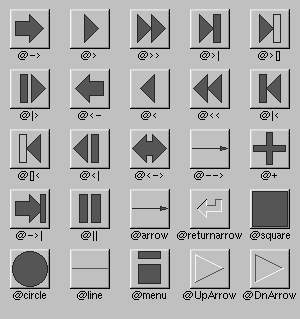
\includegraphics[scale=1]{symbols} 


 FLTK label supported symbols.


  The @ sign may be followed by the following optional ``formatting'' characters, in this order: 


 
\begin{enumerate}
\item 

 ``\#'' forces square scaling rather than distortion to the widget's shape.

\item 

 +[1-9] or -[1-9] tweaks the scaling a little bigger or smaller.

\item 

 [1-9] rotates by a multiple of 45 degrees. ``6'' does nothing, the others point in the direction of that key on a numeric keypad.


\end{enumerate}


 \emph{itype}
 -- an integer number denoting the appearance of the widget. 


  The following values are legal for \emph{itype}
: 


 
\begin{itemize}
\item 

 1 - flat box

\item 

 2 - up box

\item 

 3 - down box

\item 

 4 - thin up box

\item 

 5 - thin down box

\item 

 6 - engraved box

\item 

 7 - embossed box

\item 

 8 - border box

\item 

 9 - shadow box

\item 

 10 - rounded box

\item 

 11 - rounded box with shadow

\item 

 12 - rounded flat box

\item 

 13 - rounded up box

\item 

 14 - rounded down box

\item 

 15 - diamond up box

\item 

 16 - diamond down box

\item 

 17 - oval box

\item 

 18 - oval shadow box

\item 

 19 - oval flat box


\end{itemize}


 \emph{ifont}
 -- an integer number denoting the font of \emph{FLbox}
. 


 \emph{ifont}
 argument to set the font type. The following values are legal for \emph{ifont}
: 


 
\begin{itemize}
\item 

 1 - helvetica (same as ``Arial'' under Windows)

\item 

 2 - helvetica bold

\item 

 3 - helvetica italic

\item 

 4 - helvetica bold italic

\item 

 5 - courier

\item 

 6 - courier bold

\item 

 7 - courier italic

\item 

 8 - courier bold italic

\item 

 9 - times

\item 

 10 - times bold

\item 

 11 - times italic

\item 

 12 - times bold italic

\item 

 13 - symbol

\item 

 14 - screen

\item 

 15 - screen bold

\item 

 16 - dingbats


\end{itemize}


 \emph{isize}
 -- size of the font. 


 \emph{iwidth}
 -- width of widget. 


 \emph{iheight}
 -- height of widget. 


 \emph{ix}
 -- horizontal position of the upper left corner of the valuator, relative to the upper left corner of corresponding window. (Expressed in pixels.) 


 \emph{iy}
 -- vertical position of the upper left corner of the valuator, relative to the upper left corner of corresponding window. (Expressed in pixels.) 


 \emph{image}
 -- a handle referring to an eventual image opened with \emph{bmopen}
 opcode. If it is set, it allows a skin for that widget. 


 


\begin{tabular}{cc}
\textbf{Note about the bmopen opcode}
 \\
� &

  Although the documentation mentions the \emph{bmopen}
 opcode, it has not been implemented in Csound 4.22. 


\end{tabular}

\subsection*{Performance}


 \emph{FLbox}
 is useful to show some text in a window. The text is bounded by a box, whose aspect depends on \emph{itype}
 argument. 


  Note that \emph{FLbox}
 is not a valuator and its value is fixed. Its value cannot be modified. 
\subsection*{Examples}


  Here is an example of the flbox opcode. It uses the files \emph{flbox.orc}
 and \emph{flbox.sco}
. 


 \textbf{Example 1. Example of the flbox opcode.}

\begin{lstlisting}
/* flbox.orc */
sr = 44100
kr = 441
ksmps = 100
nchnls = 1

FLpanel "Text Box", 700, 400, 50, 50
    ; Box border type (7=embossed box)
    itype = 7
    ; Font type (10='Times Bold')
    ifont = 10
    ; Font size
    isize = 20 
    ; Width of the flbox
    iwidth = 400
    ; Height of the flbox
    iheight = 30
    ; Distance of the left edge of the flbox
    ; from the left edge of the panel
    ix = 150
    ; Distance of the upper edge of the flbox
    ; from the upper edge of the panel
    iy = 100

    ih3 FLbox "Use Text Boxes For Labelling", itype, ifont, isize, iwidth, iheight, ix, iy
; End of panel contents
FLpanelEnd
; Run the widget thread!
FLrun

instr 1
endin
/* flbox.orc */
        
\end{lstlisting}
\begin{lstlisting}
/* flbox.sco */
; Real-time performance for 1 hour.
f 0 3600
e
/* flbox.sco */
        
\end{lstlisting}
\subsection*{See Also}


 \emph{FLbutBank}
, \emph{FLbutton}
, \emph{FLprintk}
, \emph{FLprintk2}
, \emph{FLvalue}

\subsection*{Credits}


 Author: Gabriel Maldonado


 New in version 4.22


 Example written by Iain McCurdy, edited by Kevin Conder.
%\hline 


\begin{comment}
\begin{tabular}{lcr}
Previous &Home &Next \\
flashtxt &Up &FLbutBank

\end{tabular}


\end{document}
\end{comment}
